%%%%%%%%%%%%%%%%%%%%%%%%%%%%%%%%%%%%%%%%%%%%%%%%%%%%%%%%%%%%
% Document settings
\documentclass{ACGSeminar}
\usepackage{tikz}
\usepackage{svg}
\usepackage{mathtools}

\tikzset{
  root/.style     = {draw=none},
  leaf/.style     = {draw=none},
  dummy/.style    = {circle,draw},
  text-node/.style    = {rectangle, rounded corners, align=center,draw},
}

\bibliography{references}

%%%%%%%%%%%%%%%%%%%%%%%%%%%%%
% Hyphenations here
%%%%%%%%%%%%%%%%%%%%%%%%%%%%%
\hyphenation{}

%%%%%%%%%%%%%%%%%%%%%%%%%%%%%
% Title, Author, etc.

\begin{document}

\title{Efficient Ray Tracing Techniques}

\author{Dario Seyb}

\maketitle

%%%%%%%%%%%%%%%%%%%%%%%%%%%%%%%%%%%%%%%%%%%%%%%%%%%%%%%%%%%%
% Abstract

\begin{abstract}
Ray Tracing is next to rasterization the most widely used technique to generate discrete 2D images from continuous 3D scenes. Until recently ray tracing was too resource intensive to produce images in realtime, but advances in algorithms and hardware capabilities, most notably the introduction of GPGPU (General Purpose Graphics Processing Units), made near-realtime ray tracing feasible. In this report we will present some of the techniques which are used to achieve this.
\end{abstract}

\keywords{Ray Tracing, Acceleration Structures, Realtime Rendering, GPGPU}
\tableofcontents

%%%%%%%%%%%%%%%%%%%%%%%%%%%%%%%%%%%%%%%%%%%%%%%%%%%%%%%%%%%%
% Introduction

\section{Introduction} \label{introduction}
\subsection{Motivation}
Ray tracing is a technique used to synthesize photo-realistic images from a 3D scene description. This is useful in many applications, from architectural visualization, games and movies to medical imaging. While the rendered images are of very high quality, the time needed to produce even one frame of animation is usually in the minutes or hours. Big animation studios like Disney or Pixar can afford super computers to render their movies\footnote{http://www.engadget.com/2014/10/18/disney-big-hero-6/}, but this is not feasible for smaller companies or individuals. Luckily, with the advent of general purpose computation on consumer grade GPUs most people have a small super computer sitting in their PCs. The new NVIDIA GTX 1080 for example can do about 9 TFLOP/s \footnote{https://twitter.com/nvidia/status/728771223522410496}, as many as the fastest super computer in the world in 2001\footnote{http://www.top500.org/}.

Real time ray tracing is appealing, especially in the context of creative work, because it allows artist to preview changes to the scene immediately. This reduces turn around time. Where you previously had to change the position or color of a light and wait until the next day to review the difference you now can tweak scenes interactively. This leads to a lower turn around time on changes in visuals and thus higher quality results.

\begin{figure}[htb!]
  \begin{centering}
    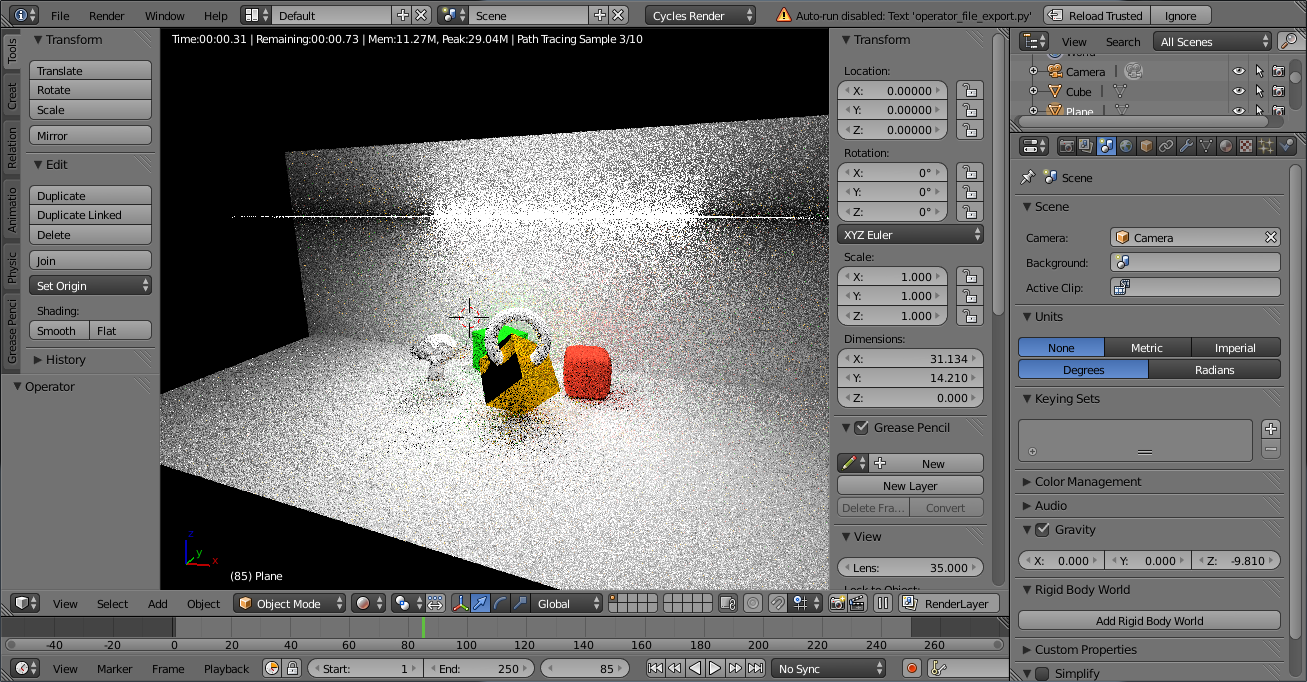
\includegraphics[width=12cm]{figures/blender_preview.png}\par
  \end{centering}
  \caption{Interactive ray traced scene view in Blender (blender.org).}
  \label{fig:blender_preview}
\end{figure}

In this report I will:
\begin{itemize}
\item Describe a state of the art ray tracing algorithm. (Section \ref{path-tracing})
\item Introduce techniques to reduce the time spent on ray-scene intersections which usually dominate the performance of ray tracing \cite{Whitted:1980}. (Section \ref{acceleration})
\item Explain how to use the fact that the algorithm is running at interactive frame rates to improve image quality. (Section \ref{noise})
\item Present an implementation. (Section \ref{gpu-adapting})
\end{itemize}


\subsection{A short history of ray tracing}
The technique of tracing rays through a scene consisting of primitives and media has been known to the computational physics community for a long time. There it is mostly used to simulate the propagation of waves (e.g. shock waves of an earthquake) through a heterogeneous medium (e.g. the interior of the earth). \cite{GJI:GJI93}

It was first described in relation to computer graphics by Arthur Appel in 1968. At the time the common method to visualize three dimensional scenes was to synthesize two dimensional line and point drawings. Appel recognized the importance of shading and shadow casting in conveying shape and spatial relations. In his paper "Some techniques for shading machine renderings of solids" he proposes a method to realize this shading by casting rays originating from the viewers' position through each pixel on the viewing plane and calculating the first point of intersection with the scene. To determine shading he casts a second ray from this intersection point to the light source. Noteworthy is that he recognized Lambert's cosine law as the basis of a physically correct model for diffuse shading of surfaces lit by a point light.
\begin{equation}
I = S (Cosine L)/D^{2}
\end{equation}
Where $I$ is the final illumination intensity, $S$ the intensity of the light source, $L$ the angle between the surface normal and the direction to the light source and $D$ the distance to the light source.
Appel's technique was very compute intensive for its time, but already illustrated the power of ray tracing to generate realistic images using a relatively simple algorithm. \cite{Appel68}

\begin{figure}[htb!]
  \begin{centering}
    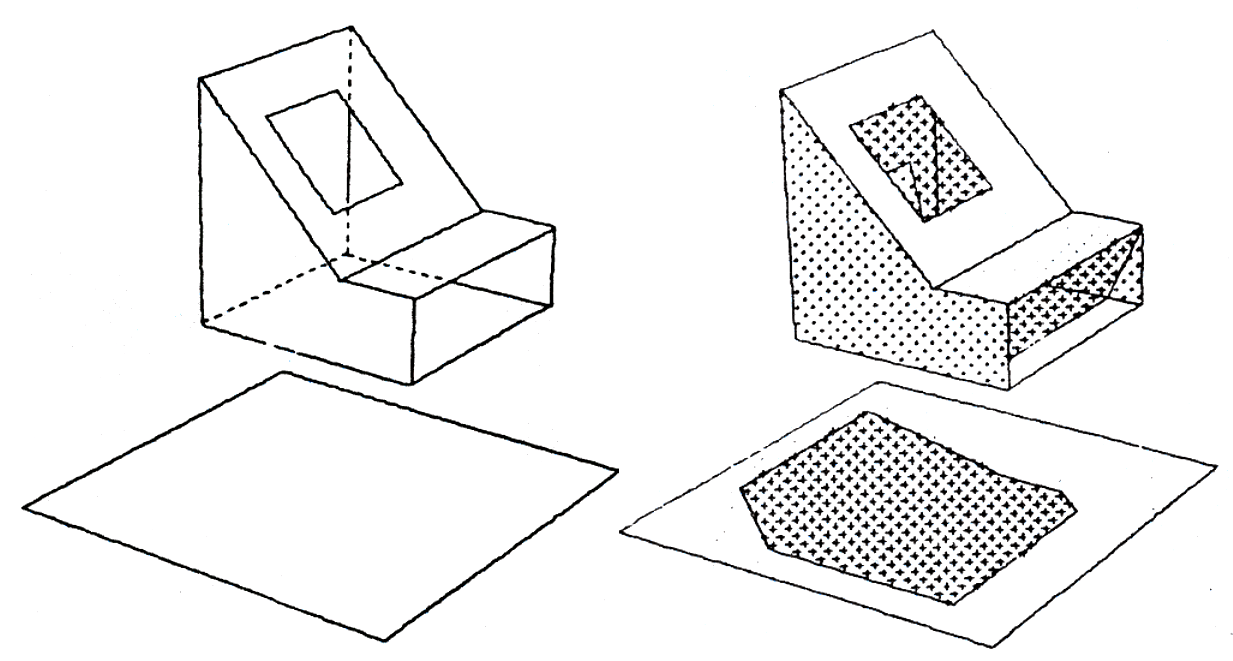
\includegraphics[width=12cm]{figures/Appel_Shading.png}\par
  \end{centering}
  \caption{Left: Unshaded Line/Point Drawing, Right: Drawing augmented with the technique introduced in \cite{Appel68}}
  \label{fig:appel_tracing}
\end{figure}

The next major contribution to ray tracing came from Turner Whitted of Bell Laboratories in 1980. In his landmark paper "An Improved Illumination Model for Shaded Display" \cite{Whitted:1980} he describes the algorithm that would become known as Recursive, or Whitted, Ray Tracing. So far ray tracing was only used to compute local illumination at the first point of intersection and the only secondary rays that were cast were shadow rays. This produced a fairly good approximation for diffuse surfaces, but was lacking in scenes with very reflective objects. Whitted took the concept of casting secondary rays and extended it to reflections and refractions. For each intersection point he proposed to not only compute a shadow ray in the direction of each light source, but also recursively compute the color of incoming reflected and refracted light. This technique produced impressive looking results, but Whitted himself acknowledged that it did not provide a solution to global illumination since objects could not act as light sources themselves and diffuse interreflections where not accounted for.

\begin{figure}[htb!]
  \begin{centering}
    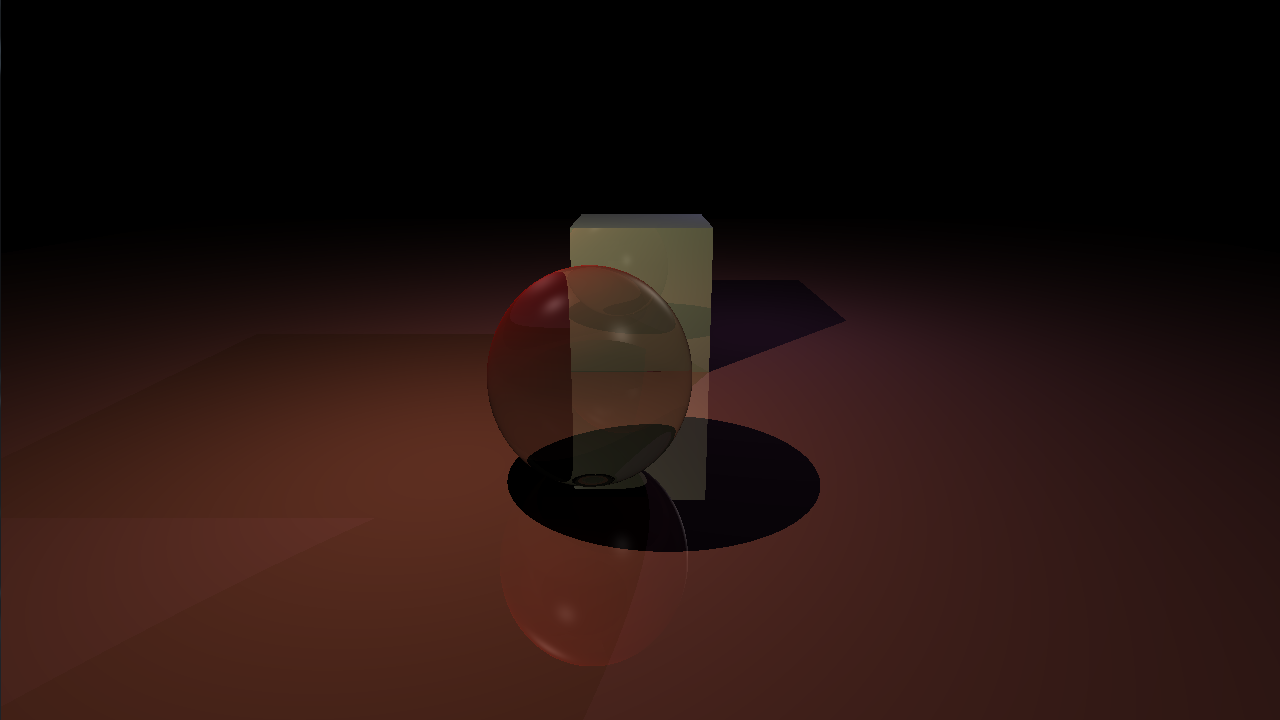
\includegraphics[width=12cm]{figures/whitted_raytracing.png}\par
  \end{centering}
  \caption{Whitted Ray Tracing implemented in the offline renderer "Zaphod" \cite{Zaphod}.}
  \label{fig:whitted-example}
\end{figure}


Over the next years many different approaches to solve this issue where proposed and in 1986 James T. Kajiya published a paper titled "The Rendering Equation"  \cite{Kajiya:1986} in which he presents an equation to describe the propagation of light in a scene. It is general enough to describe all optical phenomena we care about in computer graphics and this made it possible to classify rendering algorithms by how well they approximate a solution to the rendering equation.

\begin{equation} \label{eq:rendering-equation}
I(x,x')= \overbrace{g(x,x')}^{\mathclap{\text{Geometry Term}}}
         [
         \underbrace{\epsilon(x,x')}_{\mathclap{\text{Emission}}}
         + \underbrace{
         \int_{S}{\overbrace{p(x,x',x'')}^{\mathclap{\text{BRDF}}}
                  \overbrace{I(x',x'') }^{\mathclap{\text{Incoming light}}} dx''}
         }_{\mathclap{\text{Light reflected at $x'$ in direction $\overrightarrow{x'x}$}}} ]
\end{equation}
It describes the light transport between two points $x$ and $x'$ as a combination of emitted and reflected light at $x'$. The geometry factor describes the amount of light that actually arrives at $x$ (e.g. $g(x,x') = 0$ there is an object between the two points). To compute the reflected light we need to integrate over all directions in the hemisphere $S$ above point $x'$. 
The main difference between rendering algorithms is how they approach the evaluation of this integral. It cannot be evaluated analytically for scenes which are even remotely interesting, but the formulation of the rendering problem as an integral equation allows us to employ methods from calculus to devise new algorithms.

%%%%%%%%%%%%%%%%%%%%%%%%%%%%%%%%%%%%%%%%%%%%%%%%%%%%%%%%%%%%
% Second Section
\section{Overview over the path tracing algorithm} \label{path-tracing}
Path tracing is an algorithm which solves the integral in \eqref{eq:rendering-equation} by randomly sampling it. This process is also called "Monte Carlo integration". Each sample is represented by a list of points $(x_0, ..., x_n), x_i \in \R^3$ which for a path through space. This is similar to Whitted Ray Tracing, except that the points are randomly chosen instead of being predetermined by the reflection and refraction directions. The value 

% Path integral formulation, monte carlo methods

\section{Spacial partitioning and acceleration structures} \label{acceleration}
Going logarithmic!
\subsection{BSP and KD-Trees}

\subsection{Volume Hierarchies}

\section{Reducing Noise} \label{noise}
All stochastic sampling methods 
\subsection{Gradient-Domain Path Tracing}
Do I really want to go here? \cite{Kettunen2015sg} I'll implement everything else first and see if I have time left.
\subsection{Temporal Supersampling}


% Reference back to monte carlo, main issue of path tracing is variance expressed as noise, we need more samples. Temporal Supersampling provides these.

\section{Adapting the described algorithms to the GPU} \label{gpu-adapting}
\subsection{Accessing the GPU outside of the rasterization pipeline}
Compute shaders
% Easier integration with OpenGL (needed for TXAA)
\subsection{Hierarchical data structures on the GPU}
Use this: \cite{Karras:2012:MPC:2383795.2383801} \cite{Foley:2005}

\section{Results} \label{results}
I plan to implement everything I describe since I strongly believe computer science papers should \textbf{always} come with code.
\subsection{Images}
Pretty images rendered in real time. Link to a video.
\subsection{Timings}
Timing comparisons between the different techniques.


\begin{figure}[htb!]
  \begin{centering}
    \includegraphics[width=10cm]{figures/Output_PT_10kSPP.png}\par
  \end{centering}
  \caption{This is what my path tracer is rendering right now, but not in real time.}
  \label{fig:pathtraced}
\end{figure}

%%%%%%%%%%%%%%%%%%%%%%%%%%%%%%%%%%%%%%%%%%%%%%%%%%%%%%%%%%%%
% Bibliography

\printbibliography
\cleardoublepage

\end{document}
